\documentclass[11pt,a4paper]{article}
\usepackage[margin=1in]{geometry}
\usepackage[T1]{fontenc}
\usepackage{amsmath,amssymb,booktabs,array,tikz,xcolor,enumitem}
\usepackage[hidelinks]{hyperref}
\title{\textbf{BCJRFormer Inference ASIC Architecture}\\\large Sequential Datapath and Control Specification}
\author{Taimor Sabek \and Haiel Bader}
\date{}
\begin{document}
\maketitle

\section{Abstract}
This paper specifies a sequential inference architecture for the BCJRFormer neural decoder. The core transforms prepared received-read window features and a padding mask into one logit per decoded position. Five stages implement input embedding, position/read embedding, transformer encoding, final projection and read aggregation. A shared dot-product datapath and a reusable encoder-layer engine reduce arithmetic replication. Each stage is defined by its mathematics, storage dependencies, control sequence and completion condition. Explicit transaction protocols accommodate variable-latency memories and nonlinear arithmetic. The design preserves reference masking and aggregation semantics while identifying numerical precision and physical feasibility as validation requirements. The final research section describes candidate implementations and experiments for unresolved nonlinear operations.

\section{Scope and Architectural Overview}
The implementation boundary is BCJRFormer.forward(y, padding\_mask) in evaluation mode. Trellis/window preprocessing and outer decoding are outside the neural core. The host supplies prepared features, the original padding mask and a parameter image matching the selected configuration. Training does not execute in the ASIC.
\[
y\in\mathbb{R}^{1\times M\times N\times W\times S},\qquad
F=WS,\qquad L=MN,\qquad
p^{mask}\in\{0,1\}^{1\times M\times N}.
\]
W and S denote the two window-feature dimensions; flattening preserves software order. The hardware consumes L vectors of length F and emits N signed logits. A mask bit of one denotes padding. The baseline supports the binary-output model.
\begin{enumerate}
\item Stage 1: LayerNorm, a biased F-to-D projection and LayerNorm produce token embeddings.
\item Stage 2: learned position and read-identity embeddings are added.
\item Stage 3: pre-normalization transformer layers encode the tokens.
\item Stage 4: each encoded token is projected to one scalar logit.
\item Stage 5: read logits are combined according to the source aggregation rule.
\end{enumerate}
Real-arithmetic equations define algorithmic intent. Hardware storage conversions, widths and nonlinear approximations are specified separately; mathematical equivalence must not be confused with bit-level equality. Candidate precision values require calibration before RTL freeze.


\subsection{Dimensions and frame ownership}
One frame is active: $B=1$. Host batches are submitted sequentially. There are $M$ read slots, $N$ positions per read, $L=MN$ tokens, flattened input width $F$, feature width $D$, $H$ heads, head width $d=D/H$, and $K=N_{dec}$ layers. Require $D$ divisible by $H$. These dimensions come from the configuration matching the checkpoint; they are not learned. Weights, biases, position/read embeddings and normalization affine parameters are learned and persist between frames.
\[
t=mN+n,\qquad 0\leq m<M,\quad 0\leq n<N,\quad 0\leq j<D.
\]
Addresses and loop counters are exact unsigned integers, not quantized activations. Use terminal comparisons and explicit resets, not accidental binary overflow. A counter advances only after the corresponding accepted transaction or committed result.
The frame controller loads features and mask, runs embedding, position additions, encoder, final projection and aggregation, then transfers $N$ output logits. Stored outputs are ready before transfer; successful frame completion requires all $N$ output handshakes. Requests remain stable while stalled, and completion remains asserted until accepted. Invalid descriptors or arithmetic faults follow the error path rather than normal completion.

\section{High-Level Architecture and Stage Interfaces}
This section describes functional blocks, connections and scheduling independently of register widths and arithmetic implementation. The detailed mathematical and RTL specification follows the complete five-stage overview.

\begin{center}
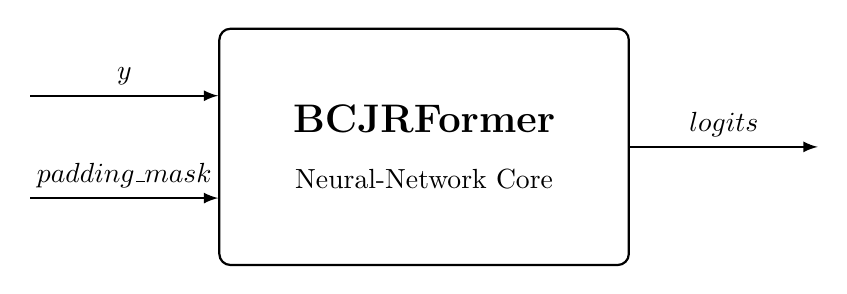
\begin{tikzpicture}[>=latex, thick]
    \node[
        draw,
        rounded corners,
        minimum width=5.2cm,
        minimum height=3.0cm,
        align=center
    ] (model) {\Large \textbf{BCJRFormer}\\[3mm]
               Neural-Network Core};

    \draw[->] (-5.0,0.65) -- (model.west |- 0,0.65)
        node[midway,above] {$y$};

    \draw[->] (-5.0,-0.65) -- (model.west |- 0,-0.65)
        node[midway,above] {$padding\_mask$};

    \draw[->] (model.east) -- (5.0,0)
        node[midway,above] {$logits$};
\end{tikzpicture}
\end{center}

\begin{center}
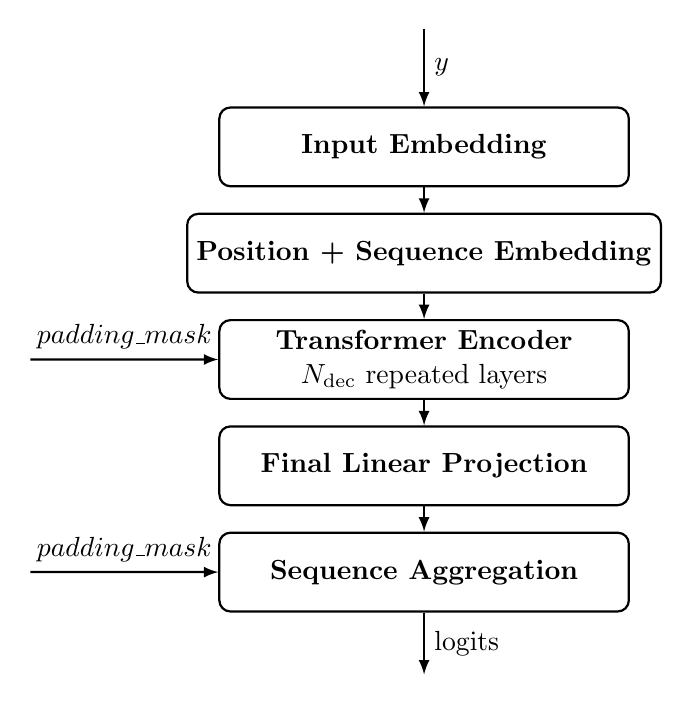
\begin{tikzpicture}[
    >=latex,
    thick,
    block/.style={
        draw,
        rounded corners,
        minimum width=5.2cm,
        minimum height=1.0cm,
        align=center
    },
    node distance=1.35cm
]
\node[block] (emb) {\textbf{Input Embedding}};
\node[block, below of=emb] (pos) {\textbf{Position + Sequence Embedding}};
\node[block, below of=pos] (tr) {\textbf{Transformer Encoder}\\$N_{\mathrm{dec}}$ repeated layers};
\node[block, below of=tr] (fc) {\textbf{Final Linear Projection}};
\node[block, below of=fc] (agg) {\textbf{Sequence Aggregation}};

\draw[->] (0,1.5) -- (emb.north) node[midway,right] {$y$};
\draw[->] (emb) -- (pos);
\draw[->] (pos) -- (tr);
\draw[->] (tr) -- (fc);
\draw[->] (fc) -- (agg);
\draw[->] (agg.south) -- (0,-6.7) node[midway,right] {logits};

\draw[->] (-5,-2.7) -- (tr.west)
    node[midway,above] {$padding\_mask$};
\draw[->] (-5,-5.4) -- (agg.west)
    node[midway,above] {$padding\_mask$};
\end{tikzpicture}
\end{center}

\subsection{Connections, storage and control ownership}
The five stages execute sequentially on one active frame. Feature data flows through the stage chain; the padding mask and model parameters follow separate paths. An arrow between stages denotes a completed tensor in shared memory, not a combinational connection or concurrent streaming pipeline.
\begin{itemize}
\item Host to Stage 1: prepared window features, flattened to $[L,F]$. Stage 1 to Stage 2: embedded tokens $e[L,D]$ in the X bank.
\item Stage 2 to Stage 3: position/read-enriched tokens $X^{(0)}[L,D]$ in the same X bank. Stage 3 to Stage 4: final encoded tokens $X^{(K)}[L,D]$.
\item Stage 4 to Stage 5: per-read logits $z[L]$, interpreted as $[M,N]$. Stage 5 to the host: aggregated logits $y[N]$.
\item Mask path: load $[M,N]$ once and retain it throughout the frame. Stage 3 interprets it as a query-row attention mask; Stage 5 uses the original read/position mask. Stages 1, 2 and 4 do not consume it for arithmetic or skip padded tokens.
\item Parameter path: the host loads and commits a matching parameter image before inference. Each active stage selects its own parameter bases; Stage 3 also selects the current layer's parameters. Parameters persist across frames.
\item Control path: the core controller commands one stage at a time. A stage returns completion only after its output writes commit; the next stage may then read those outputs. The active controller owns shared arithmetic and scratch until its command completes.
\end{itemize}

\subsection{Stage 1 overview: input embedding}
\textbf{Inputs:} feature vectors $[L,F]$; first normalization parameters $\gamma_F,\beta_F$; projection $W^{emb}[D,F],b^{emb}[D]$; second normalization parameters $\gamma_D,\beta_D$.

\textbf{Internal blocks:} token loader, LayerNorm(F), linear(F,D), LayerNorm(D), and output writer. The normalization blocks share one length-configurable engine; the linear block uses the shared dot engine.

\textbf{Architectural FSM:} IDLE/INIT, LOAD\_TOKEN, LN\_F, LINEAR\_F\_TO\_D, LN\_D, WRITE\_TOKEN, NEXT\_TOKEN, DONE. NEXT\_TOKEN loops to LOAD\_TOKEN until all L tokens are processed. Each arithmetic state commands its child controller and waits.

\textbf{Output and handoff:} $e[L,D]$. Stage 2 starts after the final embedded token is stored. Normalized input scratch is preserved until every projection output using it has been calculated.

\subsection{Stage 2 overview: position and read embedding}
\textbf{Inputs:} $e[L,D]$, learned position table $P[N,D]$ and learned read-identity table $E[M,D]$. Token index $t=mN+n$ identifies read m and position n.

\textbf{Internal blocks:} exact integer index controller, X/P/E memory readers, two sequential additions with their conversion boundaries, and in-place output writer. P and E are trained tables, not inference-time calculations.

\textbf{Architectural FSM:} INIT, READ\_X, READ\_P, ADD\_P, READ\_E, ADD\_E, WRITE, NEXT\_INDEX, DONE. Traverse feature j, then position n, then read m using terminal comparisons; NEXT\_INDEX returns to READ\_X while entries remain.

\textbf{Output and handoff:} $X^{(0)}[L,D]$ with position and read identity included. Stage 3 starts after all $LD$ feature writes commit. The mask bypasses this stage unchanged.

\subsection{Stage 3 overview: transformer encoder}
\textbf{Inputs:} $X^{(0)}[L,D]$, padding mask and K distinct layer-parameter sets. Configuration supplies D, H and K, with head width $d=D/H$; these are not learned values.

\textbf{Internal blocks:} one physical layer engine reused K times. Each layer contains LN1, self-attention, residual addition 1, LN2, FFN and residual addition 2. Original X bypasses LN1/attention into the first addition. Its result R bypasses LN2/FFN into the second addition.

\textbf{Attention subblocks:} Q/K/V projections; head-slice addressing; one QK score row and constant scaling; mask/softmax; probability-weighted V dot products; joined-head storage; output projection. Q and K feed scores; V bypasses scores/softmax and feeds the weighted-value block. FFN contains D-to-4D linear, GELU and 4D-to-D linear.

\textbf{Encoder FSM:} INIT\_LAYER, RUN\_LAYER, WAIT\_LAYER, NEXT\_LAYER, DONE. Advance the layer index and parameter bases only after a complete layer result.

\textbf{Layer FSM:} LN1\_ALL\_TOKENS, ATTENTION, RESIDUAL1\_ALL, LN2\_TOKEN, FFN\_TOKEN, RESIDUAL2\_TOKEN, NEXT\_TOKEN, DONE. The final four processing states repeat over tokens; the first three process the complete frame.

\textbf{Attention FSM:} project all Q, all K and all V; initialize head/query; compute SCORE\_ROW, SOFTMAX\_ROW and WEIGHTED\_VALUES; advance query then head; finally run OUTPUT\_PROJECTION. One row buffer is reused only after all weighted features for that row are stored.

\textbf{Output and handoff:} $X^{(K)}[L,D]$. Stage 4 starts only after the last token's second residual write in the final layer. Residual lifetimes are preserved throughout the computation.

\subsection{Stage 4 overview: final projection}
\textbf{Inputs:} $X^{(K)}[L,D]$, final weight vector $w^{final}[D]$ and scalar bias.

\textbf{Internal blocks:} token selector and the shared D-to-1 linear controller, including dot accumulation, conversion and logit writer. There is no sigmoid in this stage.

\textbf{Architectural FSM:} INIT\_TOKEN, ISSUE\_LINEAR, WAIT\_LINEAR, NEXT\_TOKEN, DONE. The linear controller owns the write; NEXT\_TOKEN repeats the command for each token without a duplicate store step.

\textbf{Output and handoff:} $z[L]$, viewed as $[M,N]$ per-read logits. Stage 5 starts after all L logits are committed. These signed scores are neither probabilities nor hard decisions.

\subsection{Stage 5 overview: read aggregation and output}
\textbf{Inputs:} $z[M,N]$ and the original padding mask $[M,N]$. No trained parameters are needed.

\textbf{Internal blocks:} path selector, valid-read counter, masked-logit accumulator, reciprocal unit, scalar multiplier/converter and output buffer. For M=1, a direct copy path bypasses counting and averaging, including masking, to preserve the software branch.

\textbf{Architectural FSM:} SELECT\_PATH; for M greater than one, COUNT\_VALID\_SLOTS, CHECK\_COUNT, RECIPROCAL, INIT\_POSITION, SUM\_READS, SCALE, WRITE, NEXT\_POSITION, DONE. The reciprocal of the frame-wide count is calculated once. NEXT\_POSITION repeats accumulation/scaling/writing until N positions are stored. The M=1 branch copies N logits and then completes.

\textbf{Output and handoff:} $y[N]$. A zero valid-read count raises an error in the averaging branch. The core subsequently transfers N buffered logits to the host and declares successful frame completion only after the last accepted output transfer. An optional downstream sign comparison can generate hard decisions.

\subsection{Controller hierarchy and interpretation of FSM states}
The core controls stages; stage controllers control reusable vector operations; linear/vector controllers control the dot or scalar arithmetic engines. These are nested control responsibilities, not additional neural-network layers. The frame sequence is LOAD\_FEATURES, LOAD\_MASK, EMBED, POSITION, ENCODER, FINAL, AGGREGATE, OUTPUT, COMPLETE, between idle periods.

A named high-level state denotes a complete operation, not one clock cycle. Its implementation may include memory-read, request, response and write-commit substates. Ready/valid handshakes accommodate stalls and variable arithmetic latency. Exact register widths, transaction details, mathematical derivations and numerical risks are specified in the following detailed design. This separation permits architectural review without requiring the reader to follow RTL-level timing first.


\section{Detailed Architecture, Mathematics and RTL Mapping}
The following five sections refine the preceding architectural overview. Each specifies the stage equations, controller operations, completion conditions and design rationale. Shared-engine protocols and implementation constraints follow the stage descriptions.

\section{Stage 1: Input Embedding}
\subsection{Interface and mathematical definition}
Input: $L$ vectors of length $F$. Output: $e[L,D]$. The two normalizations have independent learned affine parameters.

For each flattened token $x_t\in\mathbb{R}^{F}$,
\[
u_t=\operatorname{LN}_{F}(x_t),\qquad
v_{t,j}=b^{emb}_j+\sum_{r=0}^{F-1}W^{emb}_{j,r}u_{t,r},\qquad
e_t=\operatorname{LN}_{D}(v_t).
\]
LOAD\_TOKEN captures $F$ values; LN\_F runs the common normalization engine; LINEAR\_F\_TO\_D runs $D$ dots of length $F$; LN\_D uses its own affine parameters; WRITE\_TOKEN commits $D$ outputs. NEXT\_TOKEN repeats until $L$ tokens are stored. Do not skip padded tokens or overwrite the linear input scratch before all output features complete.

\subsection{Control sequence and completion}
\begin{itemize}
\item \texttt{IDLE / INIT}: Latch bases and set token index $t=0$.
\item \texttt{LOAD\_TOKEN}: Capture $F$ input features in token scratch.
\item \texttt{LN\_F}: Issue normalization of length $F$; wait for all normalized features.
\item \texttt{LINEAR\_F\_TO\_D}: Issue $D$ biased dot products of length $F$; wait for committed outputs.
\item \texttt{LN\_D}: Normalize the projected D-vector using the second gamma/beta pair.
\item \texttt{WRITE\_TOKEN}: Commit all $D$ features into the X bank.
\item \texttt{NEXT\_TOKEN / DONE}: If $t<L-1$, increment $t$ and return to LOAD_TOKEN; otherwise hold completion until accepted.
\end{itemize}

\subsection{Normalization mathematics and internal FSM}
For a vector $x$ of length $J$, with separately loaded affine parameters,
\[
\mu=\frac{1}{J}\sum_{j=0}^{J-1}x_j,\qquad
v=\frac{1}{J}\sum_{j=0}^{J-1}(x_j-\mu)^2,\qquad
g=(v+\epsilon)^{-1/2},\qquad
y_j=\gamma_j(x_j-\mu)g+\beta_j.
\]
Use the population variance (denominator $J$, not $J-1$). The reference default epsilon is $10^{-5}$. Gamma and beta are learned; mean and variance are computed for every current token.
\begin{itemize}
\item LOAD\_AND\_SUM: retain the input vector and accumulate its sum in widened storage.
\item MEAN: multiply by the configured reciprocal $1/J$; preserve the selected precision.
\item VARIANCE: reset the feature counter and sum centered squared differences in widened storage, then scale by $1/J$.
\item INV\_SQRT: add epsilon in a format that represents it, issue the scalar operation and wait for its result.
\item NORMALIZE\_WRITE: reset the counter; subtract mean, multiply by $g$ and gamma, add beta, convert and commit each output. DONE follows the final write.
\end{itemize}
The centered two-pass calculation is the proposed baseline. Its operation order can differ from a floating-point library kernel. Epsilon must not disappear through quantization. Variance, inverse square root and affine scaling are high-risk numerical areas.

\begin{center}
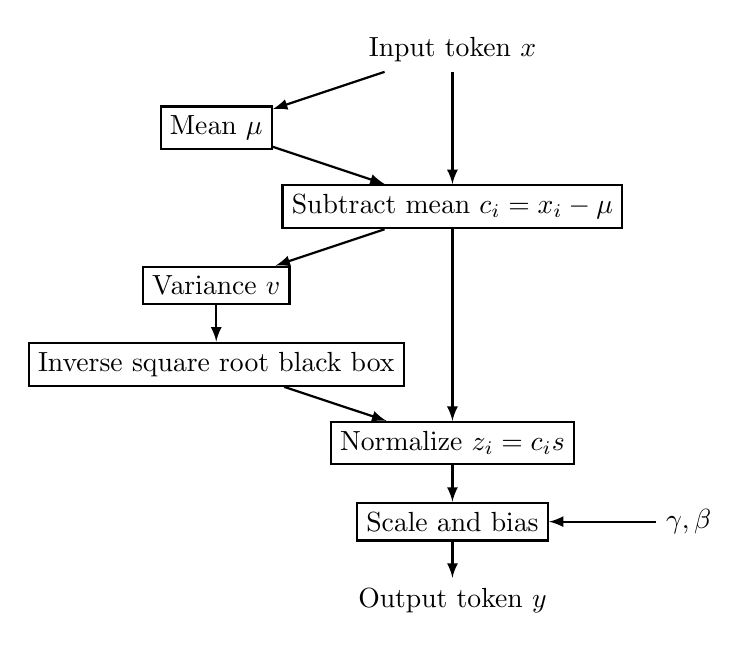
\begin{tikzpicture}[>=latex,thick,every node/.style={align=center}]
\node (x) at (0,0) {Input token $x$};
\node[draw] (m) at (-3,-1) {Mean $\mu$};
\node[draw] (c) at (0,-2) {Subtract mean\ $c_i=x_i-\mu$};
\node[draw] (v) at (-3,-3) {Variance $v$};
\node[draw] (s) at (-3,-4) {Inverse square root\ black box};
\node[draw] (n) at (0,-5) {Normalize\ $z_i=c_i s$};
\node[draw] (a) at (0,-6) {Scale and bias};
\node (p) at (3,-6) {$\gamma,\beta$};
\node (o) at (0,-7) {Output token $y$};
\draw[->] (x)--(m); \draw[->] (x)--(c); \draw[->] (m)--(c);
\draw[->] (c)--(v); \draw[->] (v)--(s); \draw[->] (s)--(n);
\draw[->] (c)--(n); \draw[->] (n)--(a); \draw[->] (p)--(a); \draw[->] (a)--(o);
\end{tikzpicture}
\end{center}

\subsection{Architectural rationale}
The first normalization conditions window features and the second normalizes the learned embedding, preserving the reference model. One length-configurable normalization engine serves both operations. Sharing the dot engine reduces arithmetic replication at the cost of latency. Projection input and output scratch must be separate because every output depends on the entire normalized input. In-place normalization is safe only after both statistics passes. Stage 2 starts after all $L$ embedded tokens are committed.

\section{Stage 2: Position and Read Embedding}
\subsection{Interface and mathematical definition}
Input: $e[L,D]$, position table $P[N,D]$ and read-identity table $E[M,D]$. Output: $X^{(0)}[L,D]$. Position $n$ locates a symbol within a read; $m$ distinguishes received reads of the same frame.

\[
a_{m,n,j}=e_{mN+n,j}+P_{n,j},\qquad
X^{(0)}_{mN+n,j}=a_{m,n,j}+E_{m,j}.
\]
P and E are loaded trained tables, not values regenerated during inference. INIT sets $(m,n,j)=(0,0,0)$; READ\_X, READ\_P, ADD\_P, READ\_E, ADD\_E and WRITE perform the two additions with separate destination conversions. With equal fractional scales, conversion need not discard fractional bits but can still saturate.
After each committed write, increment $j$ unless $j=D-1$; then reset $j$ and advance $n$. At $n=N-1$, reset $n$ and advance $m$. Finish at the last feature of read $M-1$. No runtime modulo or division is required. The padding mask bypasses this arithmetic unchanged.

\subsection{Control sequence and completion}
\begin{itemize}
\item \texttt{INIT}: Set exact integer counters $m=n=j=0$.
\item \texttt{READ\_X / READ\_P}: Capture $e_{mN+n,j}$ and trained $P_{n,j}$ through memory request/wait transactions.
\item \texttt{ADD\_P}: Compute and convert $a=e_{mN+n,j}+P_{n,j}$.
\item \texttt{READ\_E / ADD\_E}: Read $E_{m,j}$, then compute and convert $X^{(0)}_{mN+n,j}=a+E_{m,j}$.
\item \texttt{WRITE}: Commit the feature at $X_{base}+(mN+n)D+j$.
\item \texttt{NEXT\_INDEX / DONE}: Advance j, then n, then m by terminal comparisons. Repeat READ_X until the final feature commits.
\end{itemize}

\subsection{Architectural rationale}
P and E are learned during training and only read during inference; no sinusoidal generator or training datapath is required. Exact nested counters avoid runtime modulo/division and quantization errors in indexing. The two additions retain separate conversion boundaries. In-place updates require only the current feature and table values. The padding mask remains immutable and bypasses this stage.

\section{Stage 3: Transformer Encoder}
\subsection{Interface and layer equations}
For layer $k$, with its own learned parameters,
\[
U=\operatorname{LN}_{1,k}(X^{(k)}),\qquad O=\operatorname{Attn}_{k}(U),\qquad R=X^{(k)}+O,
\]
\[
T=\operatorname{LN}_{2,k}(R),\qquad G=\operatorname{FFN}_{k}(T),\qquad X^{(k+1)}=R+G.
\]
Schedule LN1\_ALL\_TOKENS, ATTENTION, RESIDUAL1\_ALL, then LN2\_TOKEN, FFN\_TOKEN and RESIDUAL2\_TOKEN for each token. Preserve original X through attention and preserve R through its FFN. In-place residual writes are safe only after both operands are captured. Layer completion follows the last residual-2 write. The encoder then selects the next layer's parameter bases, or releases $X^{(K)}$ to Stage 4. Dropout is disabled in inference.

\begin{center}
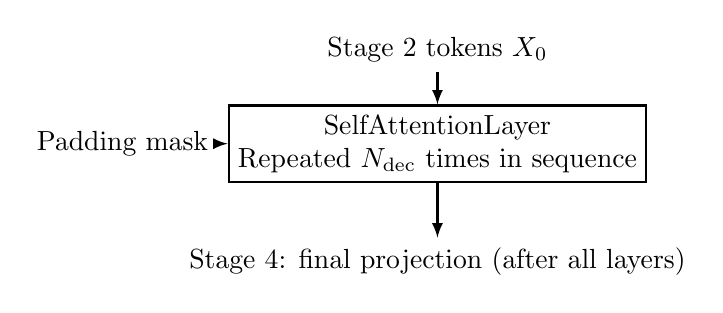
\begin{tikzpicture}[>=latex,thick]
\node (i) at (0,0) {Stage 2 tokens $X_0$};
\node[draw,align=center] (a) at (0,-1.2) {SelfAttentionLayer\\Repeated $N_{\mathrm{dec}}$ times in sequence};
\node (o) at (0,-2.7) {Stage 4: final projection (after all layers)};
\node (m) at (-4,-1.2) {Padding mask};
\draw[->] (i)--(a); \draw[->] (a)--(o);
\draw[->,dashed] (m)--(a);
\end{tikzpicture}
\end{center}

\begin{center}
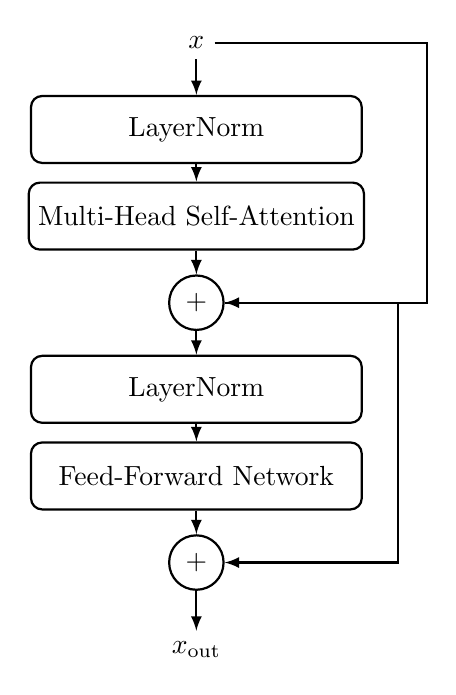
\begin{tikzpicture}[
    >=latex,
    thick,
    block/.style={
        draw,
        rounded corners,
        minimum width=4.2cm,
        minimum height=0.85cm,
        align=center
    },
    node distance=1.10cm
]
\node (xin) {$x$};
\node[block, below of=xin] (ln1) {LayerNorm};
\node[block, below of=ln1] (mha) {Multi-Head Self-Attention};
\node[circle,draw,below of=mha,minimum size=0.55cm] (add1) {$+$};
\node[block, below of=add1] (ln2) {LayerNorm};
\node[block, below of=ln2] (ffn) {Feed-Forward Network};
\node[circle,draw,below of=ffn,minimum size=0.55cm] (add2) {$+$};
\node[below of=add2] (out) {$x_{\mathrm{out}}$};

\draw[->] (xin) -- (ln1);
\draw[->] (ln1) -- (mha);
\draw[->] (mha) -- (add1);
\draw[->] (add1) -- (ln2);
\draw[->] (ln2) -- (ffn);
\draw[->] (ffn) -- (add2);
\draw[->] (add2) -- (out);

\draw[->] (xin.east) -- ++(2.7,0) |- (add1.east);
\draw[->] (add1.east) -- ++(2.2,0) |- (add2.east);
\end{tikzpicture}
\end{center}

\subsection{Control sequence and completion}
\begin{itemize}
\item \texttt{INIT\_LAYER / RUN\_LAYER / WAIT\_LAYER}: Select $k=0$ and layer-specific parameter bases; issue the layer and wait for its final residual write.
\item \texttt{NEXT\_LAYER / DONE}: For $k<K-1$, increment k and update parameter bases; otherwise release $X^{(K)}[L,D]$.
\item \texttt{LN1\_ALL\_TOKENS}: Normalize every D-feature token using the Stage-1 normalization machinery and layer-specific LN1 parameters; preserve X.
\item \texttt{ATTENTION / RESIDUAL1\_ALL}: Produce all attention outputs, then commit $R=X+O$.
\item \texttt{LN2\_TOKEN / FFN\_TOKEN / RESIDUAL2\_TOKEN}: Normalize one R token, compute its FFN and commit $X^{next}=R+G$.
\item \texttt{NEXT\_TOKEN / LAYER\_DONE}: Repeat the LN2/FFN/residual2 sequence for each token; complete the layer only after its last write.
\end{itemize}

\subsection{Architectural rationale}
A single physical layer engine executes all $K$ logical layers with distinct weights, trading throughput for reduced replication. Frame-wide Q/K/V storage ensures every key and value is available before a query starts. Row-wise attention requires score/probability scratch proportional to L rather than $L^2$. Original X survives until residual 1; token-wise FFN then limits hidden storage to $4D$. Logical bank separation simplifies lifetime verification; physical aliasing requires proof of non-overlapping use.

\subsection{Q/K/V projections and scaled score mathematics}
\[
Q_{t,j}=b^Q_j+\sum_{r=0}^{D-1}W^Q_{j,r}U_{t,r},\quad
K_{t,j}=b^K_j+\sum_{r=0}^{D-1}W^K_{j,r}U_{t,r},\quad
V_{t,j}=b^V_j+\sum_{r=0}^{D-1}W^V_{j,r}U_{t,r}.
\]
Here K as a tensor means keys; the layer count is identified by context as $N_{dec}$. The outer QKV controller selects projection and token; linear selects output feature; dot selects input term. Finish all Q tokens, then all K tokens, then all V tokens. Each projection uses all $D$ input features, not just one head slice.
\[
s_{a,i,j}=\frac{1}{\sqrt d}\sum_{r=0}^{d-1}Q_{i,ad+r}K_{j,ad+r}.
\]
For fixed head $a$ and query $i$, INIT\_KEY sets $j=0$. ISSUE\_DOT/WAIT\_DOT uses length $d$, zero initial sum, bases $Q_{base}+iD+ad$ and $K_{base}+jD+ad$, and stride one. ISSUE\_SCALE/WAIT\_SCALE multiplies by a precomputed $1/\sqrt d$; WRITE\_SCORE converts and commits. NEXT\_KEY repeats for $L$ keys. Only one score row is stored, not an $L$ by $L$ matrix.

\begin{center}
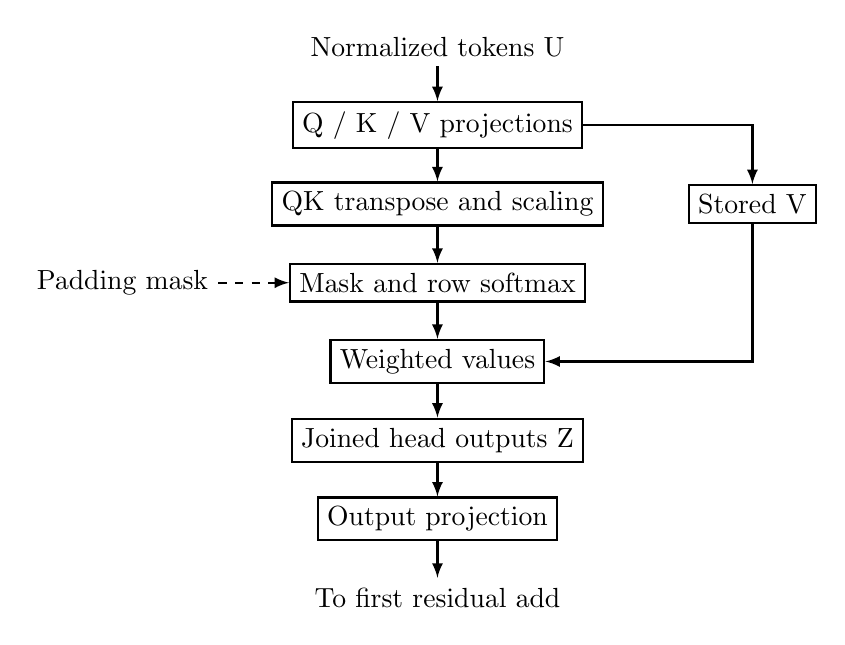
\begin{tikzpicture}[>=latex,thick,every node/.style={align=center}]
\node (i) at (0,0) {Normalized tokens U};
\node[draw] (q) at (0,-1) {Q / K / V projections};
\node[draw] (s) at (0,-2) {QK transpose and scaling};
\node[draw] (a) at (0,-3) {Mask and row softmax};
\node (m) at (-4,-3) {Padding mask};
\node[draw] (v) at (4,-2) {Stored V};
\node[draw] (w) at (0,-4) {Weighted values};
\node[draw] (z) at (0,-5) {Joined head outputs Z};
\node[draw] (p) at (0,-6) {Output projection};
\node (o) at (0,-7) {To first residual add};
\draw[->] (i)--(q); \draw[->] (q)--(s); \draw[->] (q)-|(v);
\draw[->] (s)--(a); \draw[->,dashed] (m)--(a); \draw[->] (a)--(w);
\draw[->] (v)|-(w); \draw[->] (w)--(z); \draw[->] (z)--(p); \draw[->] (p)--(o);
\end{tikzpicture}
\end{center}

\subsection{Projection and score FSMs}
QKV follows IDLE, INIT, ISSUE\_LINEAR, WAIT\_LINEAR, NEXT\_TOKEN, NEXT\_PROJECTION, DONE. INIT selects Q and $t=0$. Complete all L tokens before switching Q to K to V, resetting t on each switch. WAIT\_LINEAR means D committed writes. The final V token releases row processing.

The score-row FSM is IDLE, INIT\_KEY, ISSUE\_DOT, WAIT\_DOT, ISSUE\_SCALE, WAIT\_SCALE, WRITE\_SCORE, NEXT\_KEY, DONE. It retains head/query indices while j advances. Each score write commits before the key index changes. Precomputing $1/\sqrt d$ removes a runtime square-root operation from this path.

\subsection{Mask and softmax}
For a non-padded query row,
\[
m_s=\max_j s_j,\qquad e_j=\exp(s_j-m_s),\qquad
S_{exp}=\sum_{j=0}^{L-1}e_j,\qquad p_j=e_j/S_{exp}.
\]
CHECK\_MASK chooses the normal path or the uniform bypass. FIND\_MAX initializes from the first score, not zero. EXP\_AND\_SUM resets the counter, stores each exponential and accumulates $S_{exp}$. RECIPROCAL requests $1/S_{exp}$ once. PREPARE\_VALUE and WRITE\_PROBABILITY multiply each saved exponential by that reciprocal, convert and commit; NEXT\_ENTRY repeats until the row is ready.
The source padding shape is $[B,1,L,1]$: it masks query rows, not key columns. A padded query has all scores replaced by the same finite sentinel, yielding $p_j=1/L$ in real arithmetic. The hardware bypass uses a stored quantized $1/L$ and the same probability writer. Valid queries still attend to padded keys. This behavior must not be silently corrected. Optional static masking is outside the baseline until agreed. Quantized probabilities need not sum exactly to one; test the discrepancy. A nonpositive exponential sum raises an error.

\subsection{Softmax FSM and rationale}
The controller is IDLE, CHECK\_MASK, FIND\_MAX, EXP\_AND\_SUM, RECIPROCAL, PREPARE\_VALUE, WRITE\_PROBABILITY, NEXT\_ENTRY, DONE. Padded queries jump directly from CHECK\_MASK to PREPARE\_VALUE with uniform mode and j=0. Normal and uniform branches share the writer. Storing exponentials avoids recomputation; maximum subtraction controls the exponential range without changing real-arithmetic softmax. Scalar request/wait substates accommodate implementation-dependent latency. SOURCE\_COMPAT query masking separates hardware approximation error from algorithm changes.

\subsection{Weighted values and output projection}
\[
Z_{i,ad+r}=\sum_{j=0}^{L-1}p_j V_{j,ad+r},\qquad
O_{i,j}=b^O_j+\sum_{r=0}^{D-1}W^O_{j,r}Z_{i,r}.
\]
Weighted INIT\_FEATURE sets $r=0$. ISSUE\_DOT/WAIT\_DOT uses length $L$, probability stride one, V stride $D$, zero initial sum and unsigned-probability times signed-value arithmetic. ROUND\_SATURATE and WRITE\_RESULT commit directly to $Z_{base}+iD+ad+r$. NEXT\_FEATURE repeats for $d$ features while preserving the probability row. Only then advance query, and after the last query advance head. Joined heads need no separate copy operation.
Once every head/query result is stored, output projection issues one shared linear(D,D) command per token, waits for its writes, then advances the token. This mixes all heads. Its completion releases O to the first residual addition with original X, not normalized U.

\subsection{Weighted-value and output-projection FSMs}
Weighted-value control follows IDLE, INIT\_FEATURE, ISSUE\_DOT, WAIT\_DOT, ROUND\_SATURATE, WRITE\_RESULT, NEXT\_FEATURE, DONE. Reset r=0 per query/head; keep the probability row through all d results. Then advance query i; after its last value reset i=0 and advance head a. Output projection starts only after all heads finish.

Projection follows IDLE, INIT\_TOKEN, ISSUE\_LINEAR, WAIT\_LINEAR, NEXT\_TOKEN, DONE, waiting for D committed outputs per token. Different descriptors reuse the same dot engine for projections, QK scores and weighted values. Strided access selects the correct operand without a transpose copy. Joined-head addressing removes a separate concatenation operation.

\subsection{LN2, FFN and residual mathematics}
For the LN2 output token $T_t$,
\[
h_j=b^1_j+\sum_{r=0}^{D-1}W^1_{j,r}T_{t,r},\quad 0\leq j<4D,
\]
\[
g_j=\operatorname{GELU}(h_j)=\frac{h_j}{2}\left(1+\operatorname{erf}\left(\frac{h_j}{\sqrt 2}\right)\right),\qquad
G_{t,j}=b^2_j+\sum_{r=0}^{4D-1}W^2_{j,r}g_r.
\]
LINEAR1 runs D-to-4D with bias. GELU requests and writes every hidden feature; retain all $4D$ activated values before LINEAR2 runs 4D-to-D with bias. There is no second GELU. The exact-erf formula is the reference target, not a promise of a hardware erf implementation.
Both residual controllers capture left and right values, align their scales, add in a widened format, convert and commit. Their equations are $R_{t,j}=X_{t,j}+O_{t,j}$ and $X^{next}_{t,j}=R_{t,j}+G_{t,j}$. Feature counters advance after write completion. Residual 2 completes the current token before the layer advances.

\begin{center}
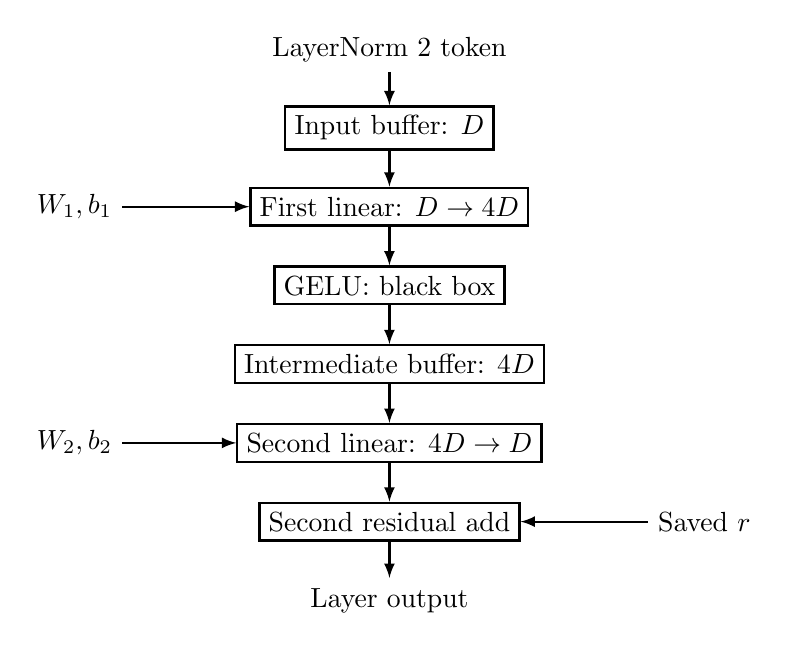
\begin{tikzpicture}[>=latex,thick,every node/.style={align=center}]
\node (i) at (0,0) {LayerNorm 2 token};
\node[draw] (b) at (0,-1) {Input buffer: $D$};
\node[draw] (l1) at (0,-2) {First linear: $D\rightarrow4D$};
\node (w1) at (-4,-2) {$W_1,b_1$};
\node[draw] (g) at (0,-3) {GELU: black box};
\node[draw] (h) at (0,-4) {Intermediate buffer: $4D$};
\node[draw] (l2) at (0,-5) {Second linear: $4D\rightarrow D$};
\node (w2) at (-4,-5) {$W_2,b_2$};
\node[draw] (a) at (0,-6) {Second residual add};
\node (r) at (4,-6) {Saved $r$};
\node (o) at (0,-7) {Layer output};
\draw[->] (i)--(b); \draw[->] (b)--(l1); \draw[->] (w1)--(l1);
\draw[->] (l1)--(g); \draw[->] (g)--(h); \draw[->] (h)--(l2);
\draw[->] (w2)--(l2); \draw[->] (l2)--(a); \draw[->] (r)--(a); \draw[->] (a)--(o);
\end{tikzpicture}
\end{center}

\subsection{FFN and residual FSMs}
FFN control issues LINEAR1 and waits for its 4D outputs; GELU\_REQ, GELU\_WAIT and GELU\_WRITE then iterate over the hidden vector. LINEAR2 starts only after every activated hidden value is stored; its last committed output permits FFN\_DONE. Preserve all 4D values because every second-layer output depends on the whole hidden vector.

Each residual uses READ\_LEFT, READ\_RIGHT, ADD\_WIDEN, ROUND\_SATURATE, WRITE, NEXT\_INDEX, DONE. Its per-feature operation is the corresponding residual equation above. Both operands are captured before an in-place write; indices advance after commitment. LN2 uses the Stage-1 normalization schedule at length D with independent affine parameters. No second GELU or inference dropout is inserted.

\section{Stage 4: Final Linear Projection}
\subsection{Interface and mathematical definition}
Input: $X^{(K)}[L,D]$. Output: one unrestricted signed logit per token, $z[L]$, for the binary target.

\[
z_t=b^{final}+\sum_{j=0}^{D-1}w^{final}_j X^{(K)}_{t,j}.
\]
INIT\_TOKEN, ISSUE\_LINEAR, WAIT\_LINEAR and NEXT\_TOKEN run D-to-1 for all $L$ tokens. The linear controller owns the logit write: there is no second STORE\_LOGIT state. The binary target uses one unrestricted logit, not a probability or a percentage.


\subsection{Control sequence and completion}
\begin{itemize}
\item \texttt{INIT\_TOKEN}: Set t=0 and select the final weight vector and scalar bias.
\item \texttt{ISSUE\_LINEAR / WAIT\_LINEAR}: Run a D-to-1 linear command on token t; wait for its destination write to $z_t$.
\item \texttt{NEXT\_TOKEN / DONE}: Increment t and repeat while $t<L-1$; release all L logits after the last write.
\end{itemize}

\subsection{Architectural rationale}
The shared biased dot product implements this projection without another arithmetic engine. The linear controller already owns conversion and writing; a second STORE\_LOGIT would duplicate work. Preserve raw logits through aggregation: averaging probabilities or making hard decisions first would change the algorithm.

\section{Stage 5: Read Aggregation and Output}
\subsection{Interface and mathematical definition}
Input: per-read logits $z[M,N]$ and original padding mask. Output: one length-N logit vector for the frame.

Let $p^{mask}_{m,n}=1$ denote padding. For $M>1$ the source aggregation is
\[
c_m=\begin{cases}1&\text{if every }p^{mask}_{m,n}=0,\\0&\text{otherwise},\end{cases}
\quad C=\sum_m c_m,\quad S_n=\sum_m(1-p^{mask}_{m,n})z_{mN+n},\quad y_n=S_n/C.
\]
COUNT\_VALID\_SLOTS and CHECK\_COUNT precede one RECIPROCAL request for $1/C$ per frame. For each position, SUM\_READS accumulates the masked numerator; SCALE multiplies by the saved reciprocal; WRITE commits $y_n$; NEXT\_POSITION repeats. Partially padded reads can contribute to the numerator without contributing to C: preserve this nonstandard source rule and confirm permitted inputs. For $C=0$, hardware reports an error, an explicit guard beyond the source's nonfinite arithmetic.
For $M=1$, copy $y_n=z_n$ directly, without masking or averaging, matching the source branch. Optional hard decisions are $\hat b_n=1$ when $y_n>0$ and zero otherwise. If a probability is needed externally, $\sigma(y_n)=1/(1+\exp(-y_n))$; sigmoid is unnecessary for the zero-threshold decision and is not added to the core.

\subsection{Control sequence and completion}
\begin{itemize}
\item \texttt{SELECT\_PATH}: For M=1, COPY_SINGLE commits N logits directly, ignoring the mask. Otherwise count valid read slots.
\item \texttt{COUNT\_VALID\_SLOTS}: Clear C; initialize each read-valid flag to one and AND it with all N inverted padding bits, then add the flag to C.
\item \texttt{CHECK\_COUNT / RECIPROCAL}: For C=0 report error; otherwise calculate and retain 1/C once per frame.
\item \texttt{INIT\_POSITION / SUM\_READS}: Set n=0; for each position clear its widened numerator and sum the M unmasked logits.
\item \texttt{SCALE / WRITE}: Multiply the numerator by the saved reciprocal, convert and commit $y_n$.
\item \texttt{NEXT\_POSITION / DONE}: Advance n and repeat SUM_READS; DONE follows N stored outputs.
\item \texttt{OUTPUT / COMPLETE (core)}: Hold output and index stable while stalled. Successful frame completion requires all N accepted transfers.
\end{itemize}

\subsection{Architectural rationale}
A frame-wide denominator permits one reciprocal calculation for all positions. Wide summation followed by a final conversion avoids repeated rounding of partial sums. Preserving the M=1 branch and partial-padding behavior maintains source compatibility; the C=0 guard explicitly reports undefined output. An optional downstream sign comparison supplies hard decisions without a sigmoid unit.

\section{Shared Arithmetic and Transaction Protocol}
For input length $I$ and output length $O$, the mathematical linear operation is
\[
y_j=b_j+\sum_{r=0}^{I-1}W_{j,r}x_r,\qquad 0\leq j<O.
\]
\begin{itemize}
\item Dot INIT\_ACC: initialize a widened accumulator to aligned bias or zero; set $r=0$.
\item READ\_INPUT\_REQ/WAIT and READ\_WEIGHT\_REQ/WAIT: capture both operands. Operand B can be a learned weight, key or value; it is not always a weight.
\item ISSUE\_MAC/WAIT\_MAC: compute $A\leftarrow A+a_rb_r$ once, capture completion, then NEXT\_TERM increments $r$ or enters DONE. DONE returns the widened result without destination narrowing.
\item Linear READ\_BIAS, DOT\_COMMAND/WAIT: select the output row and run its dot product. ROUND\_SATURATE converts once to the destination format. WRITE\_REQ/WAIT commits the result; NEXT\_OUTPUT advances $j$ or completes.
\end{itemize}
The source vector must survive all $O$ dot products. Logical projections reuse this engine sequentially; diagram branches do not imply parallel multipliers. Memory adapters and scalar engines have request/wait substates, so a named arithmetic state is not necessarily one clock cycle.

\subsection{Frame-level controller}
The core follows IDLE, LOAD\_FEATURES, LOAD\_MASK, EMBED, POSITION, ENCODER, FINAL, AGGREGATE, OUTPUT, COMPLETE. Each compute state issues one stage command and waits for completion. Input counters advance only on accepted transfers and validate the final-element marker. Parameters must be committed before accepting a frame. OUTPUT drains all N stored logits under ready/valid backpressure; COMPLETE holds the result status until accepted, then returns to IDLE. Parameter storage persists between successful frames. Reset invalidates configuration and frame state. A latched error stops new work, drains accepted transactions and returns an error completion rather than a successful result.

\subsection{Dot and linear state transitions}
Dot FSM: IDLE -> INIT\_ACC -> READ\_INPUT\_REQ -> READ\_INPUT\_WAIT -> READ\_WEIGHT\_REQ -> READ\_WEIGHT\_WAIT -> ISSUE\_MAC -> WAIT\_MAC -> NEXT\_TERM -> DONE. IDLE captures one command on acceptance. INIT\_ACC sets term=0 and loads the aligned bias or zero. Each REQ holds its payload until accepted; each WAIT captures only an accepted response. ISSUE\_MAC requests A + operandA*operandB once; WAIT\_MAC captures the updated accumulator. NEXT\_TERM increments and returns to READ\_INPUT\_REQ while term+1<length, otherwise enters DONE. DONE holds the widened result until accepted, then returns to IDLE. READ\_WEIGHT is the generic second operand: it can instead read K or V. Operand registers, accumulator, bases, strides, length and mode are retained across waits. The engine does not round or write the projection destination itself.

Linear FSM: IDLE -> INIT\_OUTPUT -> READ\_BIAS\_REQ -> READ\_BIAS\_WAIT -> DOT\_COMMAND -> DOT\_WAIT -> ROUND\_SATURATE -> WRITE\_REQ -> WRITE\_WAIT -> NEXT\_OUTPUT -> DONE. INIT\_OUTPUT sets j=0. Bias is aligned to the accumulator format. DOT\_COMMAND supplies source base, weight-row base, input length and initial accumulator; it waits for command acceptance. DOT\_WAIT captures one completed widened sum. WRITE\_REQ holds address/data until accepted; WRITE\_WAIT waits for commitment. NEXT\_OUTPUT increments j and returns to READ\_BIAS\_REQ while j+1<O, otherwise enters DONE. For projection, I=O=D and destination is selected\_bank\_base+tD+j. DONE holds token completion until accepted. It means D committed writes, not one completed MAC.

\section{RTL Specification and Implementation Constraints}
\subsection{Proposed configuration}
One frame at a time, B=1. Compile-time parameters: N encoded positions, M read slots, F window features, D model width, H heads, K encoder layers; L=M*N and d=D/H. Require all dimensions positive and D divisible by H. Preserve the general M>1 path even if the first test uses M=1. N and F must be selected with the dataset/checkpoint, not guessed from the model YAML.

Use sequential arithmetic and one exclusive shared dot-product engine. Keep all Q/K/V vectors for a layer, but only one attention score row. Do not parallelize layers or frames in this baseline. The same encoder hardware iterates over layers with different parameter bases.

Numerical proposal, pending calibration: signed 16-bit stored activations and weights with 10 fractional bits (range -32 to 31.9990234375). Standard linear and QK dot products use a signed 48-bit accumulator with 20 fractional bits. Products are exact 32-bit signed values before extension. Biases are stored at 16/10 and shifted left by 10 before accumulator initialization. The same physical engine also supports a 24-bit unsigned probability times a 16-bit signed value; zero-extend probabilities before multiplication and use a signed 64-bit accumulator with 32 fractional bits for weighted values. Set the physical accumulator width to 64 and sign-extend the standard 48-bit mode while checking its declared range. Round to nearest, ties to even, then saturate on narrowing. Record saturation and accumulator-overflow flags. This format is a starting experiment, not an accuracy claim. Wider formats and per-tensor scales may be needed.

LayerNorm means use signed 32-bit/20-fraction values. Centered differences use signed 40-bit/20-fraction values, with 80-bit full products and 96-bit/40-fraction variance accumulation before division by V. Variance plus epsilon is unsigned 48-bit/32-fraction at the rsqrt interface. Represent softmax exponentials and probabilities in unsigned 24-bit/22-fraction format, with a 64-bit/22-fraction sum. Score rows use signed 48-bit/20-fraction values, retaining QK precision through scaling (not 16-bit narrowing). All reductions check overflow. Compile-time bounds: V<=65535, L<=65535, and d<=65535; reject larger configurations. These are proposed numeric bounds, not practical SRAM capacity targets. Precision adapters are explicit operations; epsilon is round(1e-5 * 2\textasciicircum{}32)/2\textasciicircum{}32 and must not round to zero. Implementing the wide scalar path serially is allowed; it is distinct from the shared matrix dot engine. Accuracy must be established by bit-accurate tests before RTL is frozen.

\subsection{Scalar arithmetic and constants}
For the proposed bit-accurate baseline, constants are elaboration-time values rounded to nearest, ties to even: 1/F and 1/D use unsigned40/32; 1/sqrt(d) uses unsigned32/30; the uniform attention probability 1/L uses unsigned24/22. They are not learned weights. Runtime 1/C uses the reciprocal unit after checking C>0.

LayerNorm sum is signed48/10. Multiply by unsigned40/32 (zero-extended for signed arithmetic), retaining a signed89/42 product, then round to signed32/20 mean. Center by extending the input to signed40/20. Accumulate full centered squares in unsigned96/40; multiply the variance sum by unsigned40/32 using a full unsigned136/72 intermediate, then round to unsigned48/32 and add epsilon. Such wide intermediate registers may be implemented by a serial scalar datapath; they do not travel through the 96-bit memory adapter. Multiply centered signed40/20 by zero-extended rsqrt unsigned32/20 to signed73/40; round to signed32/20 normalized value. Multiply by signed16/10 gamma to signed48/30, add beta extended to signed49/30, then round/saturate to signed16/10. All intermediate range violations raise numerical error rather than silently wrapping.

Scale signed48/20 QK scores by unsigned32/30 using signed81/50 full multiplication, then round to signed48/20. Subtract the row maximum in signed49/20; compare with -16 before narrowing the retained exp input to signed48/20. Normalize unsigned24/22 exponentials with unsigned40/32 reciprocal through unsigned64/54, then round to unsigned24/22. Independent probability rounding need not sum exactly to one; measure that error in verification. Aggregate unmasked logits using signed48/10 sum; multiply by runtime unsigned40/32 reciprocal into signed89/42, then round/saturate to signed16/10. Position and residual additions use signed17/10 before narrowing. The final logit storage proposal is signed16/10. These are explicit draft rounding points, not proof of equivalence to floating-point inference.

All modules use clk and synchronous active-high rst. On reset: deassert output valid, clear busy/counters/ownership and invalidate configuration/frame state. Memory contents need not clear because valid flags prevent reads of stale data.

Commands use cmd\_valid/cmd\_ready. Capture descriptors only when both are high. Only one command is outstanding per engine. Results use rsp\_valid/rsp\_ready with rsp\_error; hold response and error stable until accepted. A response indicates all commanded writes have committed, not merely that arithmetic has started. Address/data requests and responses each use ready/valid. Counters advance on accepted work or completed results, never on an unaccepted request. If stalled, hold payload/address/control stable. No timeout is inferred; a diagnostic watchdog is optional and outside the baseline behavior.

Arithmetic primitives use req\_valid/req\_ready, operands and operation tag, followed by rsp\_valid/rsp\_ready, result and error. Latency may vary; controllers wait for the response. One outstanding request avoids tag-reordering logic. Errors latch at top level, stop new requests, drain any accepted transaction, and produce one error completion. Reset is required before retry after an error in this initial proposal.

\subsection{Top-level ports and load order}
bcjrformer\_core: clk, rst; parameter-write channel \{valid,ready,addr,data\}; parameter\_commit; frame command \{valid,ready\}; feature input \{valid,ready,data,last\}; mask input \{valid,ready,bit,last\}; logit output \{valid,ready,data,index,last\}; completion \{valid,ready,error\}; busy; numerical-status flags.

Parameter writes are accepted only in IDLE before a frame, sequentially from address zero, with the exact manifest length. Reject out-of-order, duplicate and out-of-range addresses. parameter\_commit is accepted only after all expected words have committed; any new load invalidates the old image. Host supplies the matching configuration manifest; a checksum is a verification/host responsibility. No run-time dimension changes.

parameter\_commit is a one-cycle strobe legal only while IDLE after the last parameter write response; it has no ready signal. An illegal strobe latches a protocol error and requires reset. Frame-command ready is high only for a committed image with no outstanding parameter transaction and no parameter write/commit presented that cycle. Parameter writes take priority over frame commands. Top-level data widths are 16 for weights/features/logits, one for mask/last/valid/ready/error/busy, PARAM\_ADDR\_W for parameter address, and max(1,ceil(log2(N))) for output index. Feature and mask counters are sized from their complete bank lengths, not the 16-bit vector descriptor count. Status bits distinguish saturation (sticky, nonfatal), arithmetic overflow/domain error, and protocol error (fatal). Saturation clears at each accepted frame; fatal status clears only on reset.

After frame command acceptance: load L*F features in m,n,f order, then L mask bits in m,n order. Check last exactly at the specified final element. Early or missing last is a frame error. No feature/mask overlap is required. Compute starts after both loads. Output N logits in n order with last on n=N-1. Completion is asserted after the final output transfer; output backpressure must not discard or duplicate logits.

\subsection{Module hierarchy and contracts}
\begin{itemize}
\item Module -- Inputs / read ownership -- Outputs / completion
\item core\_ctrl -- Complete frame and parameter image -- Commands the five stages and emits logits
\item embedding\_ctrl -- Features [L,F]; three normalization/linear parameter sets -- Stage 1 X [L,D]
\item position\_ctrl -- X, P[N,D], E[M,D] -- In-place X+P+E [L,D]
\item encoder\_ctrl -- X and mask; layer parameter base -- K layers completed, X [L,D]
\item layer\_ctrl -- One layer input X [L,D] -- Updated layer output [L,D]
\item layernorm\_ctrl -- Vector length V (F or D), source/destination addresses, gamma/beta bases -- One V-element normalized vector
\item linear\_ctrl -- Input length I, output length O, vector/weight/bias/output bases -- O outputs, bias included
\item attention\_ctrl -- All normalized tokens U [L,D], padding mask, optional static mask -- O [L,D] after output projection
\item softmax\_ctrl -- One L-element score row plus mask tags -- One L-element probability row
\item ffn\_ctrl -- One normalized token [D], FFN parameters -- One FFN token [D]
\item residual\_ctrl -- Two D-element vectors, destination -- D committed sums
\item final\_ctrl -- Encoder tokens [L,D], final weights/bias -- Per-read logits [L]
\item aggregation\_ctrl -- Logits [M,N] and original mask [M,N] -- N logits and denominator status
\item dot\_engine -- I, operand-memory descriptors, accumulator initial value -- One widened dot product
\item parameter\_mem -- Read address or idle-time host write -- Parameter data / accepted write
\item scratch\_mem -- Exclusive owner requests -- Read/write completion
\item exp\_unit, reciprocal\_unit, rsqrt\_unit, gelu\_unit -- Numeric requests under the common protocol -- Numeric result/error with bounded input domain
\end{itemize}


Address widths are max(1,ceil(log2(depth))) for each bank. Counter widths must represent the terminating count (ceil(log2(count+1))), or use last-index comparisons without overflow. Parameter arithmetic uses elaboration-time constants and checks total address range.

Descriptor register contracts: layernorm=\{V,src,dst,gamma\_base,beta\_base\}; linear=\{I,O,src,dst,W\_base,b\_base\}; residual=\{V,left,right,dst\}; attention=\{L,D,H,U\_base,O\_base,Q\_base,K\_base,V\_base,Z\_base,layer\_param\_base\}; dot=\{I,A\_base,A\_stride,B\_base,B\_stride,mode,acc\_init\}; softmax=\{L,score\_base,prob\_base,padded\_query\}. Counts are 16-bit unsigned under the declared bounds; every descriptor count, including FFN length 4D and layer count K, must fit 1..65535. Bases and strides are BANK\_ADDR\_W unsigned; products of dimensions and all memory-size calculations use at least 64-bit elaboration/host arithmetic and must fit their bank. Descriptors are latched on command acceptance and immutable until completion. mode selects signed16xsigned16/20-fraction or unsigned24xsigned16/32-fraction accumulation. acc\_init is signed64 in the selected binary point.

Memory requests carry valid, ready, write, bank, address, data and format; write responses acknowledge commitment and read responses carry data. Native banks use their declared width; the common adapter payload is 96 bits with unused upper bits zero on writes and canonical sign/zero extension on reads. Bank/format mismatches raise errors. Parameter words remain 16 bits except static-mask bits and the host-independent wider constants. No byte enables or burst ordering are required for the draft.

\subsection{Memory ownership and lifetime}
\begin{itemize}
\item Storage -- Elements -- Lifetime / owner
\item --- -- ---: -- ---
\item Feature memory -- L*F -- Load through completion of embedding
\item Padding bits -- L -- Whole frame; immutable during compute
\item X residual bank -- L*D -- Holds original layer input until attention residual addition; then holds r until FFN residual addition
\item U normalized bank -- L*D -- LayerNorm 1 output until Q/K/V creation completes
\item Q, K, V banks -- 3*L*D -- One complete attention layer
\item Z bank -- L*D -- Concatenated weighted-head outputs until output projection completes
\item Attention output bank -- L*D -- Output projection until residual addition
\item Token scratch -- max(F,D) -- Normalization or FFN input, exclusive sequential use
\item FFN hidden -- 4D -- One token's GELU outputs until second linear completes
\item Vector result scratch -- max(D,4D) -- Linear/normalization result, assigned exclusively
\item Score, exponential, probability rows -- 3L -- One head/query row; each has its own numeric format
\item Logits -- L -- Final projection through aggregation
\item Aggregated output -- N -- Aggregation through host transfer
\end{itemize}


Add scalar scratch registers for mean, centered difference, squared value, variance, row maximum, widened row sum, reciprocal and loop indices. Optional static-mask storage contains L*L bits and is immutable during a frame. All listed banks are logically separate in this conservative draft; capacity reduction through aliasing requires a later lifetime proof.

Stage 1 uses token scratch for F-element input normalization in place: both statistics passes finish before any output overwrites its corresponding input. The F-to-D projection writes separate vector result scratch, followed by in-place D-element normalization there, then copies D results to X. FFN input scratch and hidden/result banks remain separate while needed. No linear command may alias its source and destination when future outputs still need the original source vector.

Proposed single-port synchronous banks, abstracted behind request/response adapters. Dot engine reads operand A, captures it, then operand B, captures it, then issues MAC and waits. It does not assume two reads per cycle. Banks may later be dual-ported without changing controller contracts. No other controller uses shared arithmetic or scratch while an owner command is outstanding.

Residual writes are in-place only after both operands at that address have been captured. All Q/K/V must exist before attention score evaluation. All head results for a token must exist before its output projection. All attention outputs are computed before overwriting X with first residual sums. FFN is then processed token by token; each r token survives until its own second residual addition commits.

Parameter tensors use software Linear layout W[out,in], row-major: base+out*I+in. Token address=t*D+i; t=m*N+n. Head component address=t*D+a*d+r. P address=n*D+i, E address=m*D+i. Layer parameters have distinct base addresses. A generated parameter manifest must list all tensor bases, shapes, formats and checksums. Parameter count in 16-bit words is 2F + DF + 3D + ND + MD + K*(12D\textasciicircum{}2+13D) + D+1: Stage 1 has two LayerNorms and an F-to-D linear; each encoder layer has four D-to-D projections, two FFN projections, and two LayerNorms; the final projection has D weights and one bias. Optional mask bits and numeric constants are separate. Sum bank sizes using their individual widths to obtain bit capacity once F,N,M,D,H,K are selected.

\subsection{FSM conventions}
Every ISSUE state waits for request acceptance, every WAIT state waits for accepted completion, and every WRITE waits for memory acceptance/completion. The compact sequences below expand to those states where needed. No transition proceeds on busy alone. All terminal states hold response until accepted. Primitive errors take the error path described above.

On accepted command, clear the command's loop indices and reduction registers; latch immutable lengths and bases. Each nested-loop restart clears its inner index and accumulator before issuing work. Linear output accumulators initialize from the current bias, never the previous output. LayerNorm sum and variance sum clear separately before their passes; softmax maximum initializes from the first score (not zero), and exp sum clears before its pass. Aggregation clears C at frame start, a slot-valid flag at each new slot (initialized true), and the numerator at each new position. The slot-valid flag ANDs the inverse mask bit for all N positions before contributing to C. Capture a memory or primitive result only on its response handshake; advance the associated index only once that operation's dependent write, if any, commits.

For attention, inner score-key index j resets for each (head a, query i); dot term index resets for each key. Weighted-value component r resets for each query; its dot term runs over j. On query completion: if i+1<L, increment i; else set i=0 and, if a+1<H, increment a; otherwise proceed to output projection. Output-token index restarts at zero. For the layer FFN loop, t restarts at zero after the first residual pass; for each next layer, all token/head/feature indices restart and only the parameter base advances. Every compact terminal DONE returns to command-ready IDLE only after response acceptance.

\subsection{Arithmetic black-box contracts}
\begin{itemize}
\item Unit -- Domain and behavior -- Completion and unresolved choices
\item rsqrt -- Unsigned48/32 input in [quantized epsilon,4096]; unsigned32/20 output -- Error on invalid domain. Proposed relative error <=2\textasciicircum{}-12; method unselected
\item GELU -- Signed16/10 input in [-32,32); signed16/10 output approximates x*Phi(x) -- Proposed absolute error <=2\textasciicircum{}-9. Below -8 return 0, above 8 return input; verify endpoints and saturation
\item exp -- Signed48/20 input difference <=0; unsigned24/22 result -- exp(0)=1; below -16 return 0. Proposed absolute error <=2\textasciicircum{}-20 over [-16,0]; error for positive input
\item reciprocal -- Positive denominator in [1,65535], unsigned64/22 or integer converted to that format; unsigned40/32 output -- Error on zero/out-of-range. Proposed relative error <=2\textasciicircum{}-12 plus one output LSB
\item MAC -- Signed16xsigned16 or unsigned24xsigned16 as selected by mode -- 64-bit physical accumulation, mode-specific range checks; error flag on overflow
\end{itemize}


These are proposed acceptance targets for a primitive implementation, not measured guarantees. Numeric-unit responses arrive within a configurable proposed watchdog bound of 1024 cycles after acceptance, excluding response backpressure; timeout raises an implementation error only if watchdog is enabled. Before choosing a slow serial implementation, either meet this bound or explicitly revise the contract. The core itself has no fixed frame-cycle promise. Softmax clipping can change results for very large L; evaluate its row-sum and logit impact rather than relying only on scalar exp error.

No hardware method is implied by these contracts. RTL stubs must not synthesize placeholder math and be reported as completed computation. Numerical adapters, constants and saturation boundaries must be included in the golden fixed-point model.

\subsection{Verification and implementation gates}
1. Establish exact repository revision, configuration, checkpoint, tensor shapes and parameter manifest. Compare float intermediate tensors at every block boundary.
2. Build a bit-accurate model using the proposed formats, operation order, rounding and primitive approximations. Measure saturation and output/logit error; evaluate decoding impact before approving widths.
3. Test M=1 and M>1, K=1 and K>1, head indexing, distinct per-layer parameters, zero variance, large values, fully padded query rows, partially padded slots and C=0 guard. Explicitly compare source-compatible masking.
4. For each RTL unit, randomize ready stalls and memory/primitive latency; verify stable outputs during stalls, no duplicate requests, correct counter termination and reset during each wait state.
5. End-to-end compare intermediate memories, then final logits; prove shared-resource exclusivity and residual data lifetime. Test invalid parameter/frame loads.
6. Run small-block synthesis early, then integrated synthesis only after functionality. Capture tool version, constraints, library, area, timing, warnings and unconstrained paths. Physical implementation is included only if required by the agreed BSc finish line.

\subsection{Numerical observations}
Record the floating-point reference, widened fixed-point intermediate and stored fixed-point value separately. The widened value may already include upstream quantization error. Capture indices, formats, rounding-change, saturation and overflow flags once per accepted conversion event, not repeatedly during stalls. Simulation observation needs no additional compute FSM state. Optional on-chip snapshots require a separately bounded buffer and readout design; no compute stall or wide-result bypass is assumed.
The remaining arithmetic black boxes are GELU, exponential, reciprocal and inverse square root, including their reduction/scaling precision. Their request/response boundaries and schedule are specified; their arithmetic implementation is not frozen. Accumulator widths, memory mapping, clock target and resource feasibility require measurement and synthesis. Earlier numeric contracts are experimental candidates, not demonstrated accuracy or latency guarantees.

\subsection{Snapshot records and physical feasibility}
The verification architecture requires add simulation observation and numerical-status signals at existing conversion/commit events, without adding computation FSM states. This is a verification requirement, not an implemented trace system. Compare three values: original Python floating-point reference; wide fixed-point result before conversion; stored result after conversion. The wide fixed-point result is not the original floating-point result because upstream inputs, weights and operations may already be quantized.

Each trace record includes frame/layer/block/projection/token/head/feature or term location as applicable, before and after raw integer values with widths/signedness/fractional bits, rounded\_changed, saturated, overflow, and a single valid event. rounded\_changed means rounding altered the represented value before clipping; saturated means clipping to a representable bound; overflow means an intermediate exceeded its declared range. Flags can coexist and must not be conflated. Capture source context and conversion flags with the result, preserve them across stalls, and log a stored result once at its accepted commit event, not on every waiting cycle. Correlate conversion and write events when they occur in different states.

Verification workflow: run the float reference and a bit-accurate hardware model on identical inputs/parameters; compare intermediate tensors and final logits; then require RTL simulation to match the bit-accurate model exactly. Measure local conversion error separately from accumulated error relative to float. Precision and nonlinear approximation targets are not approved until saturation, error and decoding impact are evaluated. A comparison viewer should show location, float reference, decoded pre/post values, raw formats, error and flags, with filters for rounded/saturated/overflow events. Do not fabricate reference values when a matching trace is unavailable.

Detailed simulation traces live in the testbench, not synthesized on-chip RAM. Optional silicon snapshots need selection registers, bounded capture storage, valid/full or dropped-event indication and a readout interface. If enabled, the proposed debug capture must not backpressure computation: stop capturing or flag drops when full. Per-block counters and first-event location are candidates to size separately. On-chip capture and a wider-result bypass are not included in the proposed baseline; a bypass would require compatible downstream formats. No extra rounding/saturation state is introduced solely for debugging.

Architecture must budget bank capacity, ports, bandwidth, resource sharing and rough memory/engine locality now; exact macro and cell placement belongs to physical design. Logical banks need not map one-to-one to SRAM macros. Q/K/V capacity alone is 3LDw bits at storage width w; add U, residual, weights and all other banks before estimating a fit. Confirm target technology/library, SRAM availability, actual model dimensions and precision. Use early synthesis and later floorplanning feedback to revise the architecture if necessary. The sequential schedule does not establish physical feasibility.

\section{Design Review Decisions}
This architecture specifies proposed behavior, not completed RTL or measured silicon. The following decisions are required before implementation freeze.
\begin{itemize}
\item Confirm configuration and usable checkpoint, binary output, query-row masking, static-mask exclusion, partial-padding policy and C=0 guard.
\item Accept the sequential shared-engine baseline and define latency, throughput, clock, area and power objectives.
\item Select target technology, available SRAM macros and physical-design scope; verify total storage and access requirements.
\item Agree numerical tolerances, decoding-performance criteria and held-out datasets before choosing formats and nonlinear implementations.
\item Confirm required RTL, verification, synthesis and reporting deliverables. Arithmetic placeholders do not count as completed computation.
\end{itemize}
\section{Source References}
The software mapping is based on repository revision \texttt{c7cf84e218730f4583e79af6dd876b04384d33f5}. Revalidate the mapping if the selected software reference changes.
\begin{itemize}
\item Model boundary, embedding and aggregation: \url{https://github.com/streit-julian/BCJRFormer/blob/c7cf84e218730f4583e79af6dd876b04384d33f5/bcjrformer/models/bcjrformer.py}
\item Encoder primitives: \url{https://github.com/streit-julian/BCJRFormer/blob/c7cf84e218730f4583e79af6dd876b04384d33f5/bcjrformer/models/modules.py}
\end{itemize}

\section{Numerical Research Findings and Black-Box Validation Plan}
The following literature and course-material analysis motivates candidate arithmetic implementations. Published results concern the cited systems; the BCJRFormer numerical contracts require independent validation.

\subsection{Course material and reference semantics}
The local compression tutorial, ee046211\_tutorial\_10\_compression\_pruning\_amp.pdf (28 pages, especially pages 8--14), motivates calibration observers, static quantization, per-channel weights and quantization-aware training. Its dynamic-quantization software recommendations are not an ASIC implementation recipe. AMP and gradient scaling concern floating-point training, not integer-only inference.
DL10\_Transfer learning.pptx (62 slides) provides background on transfer learning and fine-tuning, but does not specify fixed-point GELU, softmax or normalization hardware. It may help if later adaptation or quantization-aware fine-tuning is required.
The repository declares PyTorch 2.4.0+cu118. Its LayerNorm uses population variance and default epsilon $10^{-5}$; nn.GELU() defaults to the erf formulation, not the optional tanh approximation. PyTorch 2.4 CPU softmax uses a maximum shift, exponential, sum and reciprocal multiplication. Fix the actual checkpoint, runtime, device, dtype and arithmetic settings for the reference; different kernels need not produce identical floating-point bits.
\begin{itemize}
\item PyTorch version-matched GELU implementation: \url{https://raw.githubusercontent.com/pytorch/pytorch/v2.4.0/aten/src/ATen/native/cpu/Activation.cpp}
\item PyTorch version-matched softmax implementation: \url{https://raw.githubusercontent.com/pytorch/pytorch/v2.4.0/aten/src/ATen/native/cpu/SoftMaxKernel.cpp}
\item LayerNorm mathematical definition: \url{https://docs.pytorch.org/docs/2.14/generated/torch.nn.LayerNorm.html}
\end{itemize}

\subsection{Relevant papers: methods and evidence level}
\begin{itemize}
\item I-BERT (ICML 2021) demonstrates integer-only Transformer inference using polynomial GELU/exponential approximations and iterative integer square root, with integer matrix operations and wider nonlinear arithmetic. Its evaluation is software/GPU, not an ASIC chip. Its reported GELU error of about 0.018 and exponential approximation gap of about 0.0019 do not establish our much tighter candidate targets of $2^{-9}$ and $2^{-20}$. Reuse the ideas, then measure against our formats and task. \url{https://proceedings.mlr.press/v139/kim21d.html}
\item SwiftTron (IJCNN 2023) describes an integer Transformer accelerator with requantization and nonlinear units, evaluated through 65 nm synthesis and gate-level analysis, not measured silicon. Useful ideas include multiplier/shift rescaling and handling residual scale alignment. Its architecture and numerical settings cannot be transferred to our pre-normalization model without checking semantics and error. \url{https://arxiv.org/pdf/2304.03986}
\item ITA (ISLPED 2023) provides an attention accelerator with hardware-friendly softmax and an open implementation. Its 22 nm results are physical-implementation/post-layout estimates rather than measured-chip results. Shift-based exponential approximations and streaming normalization rely on the paper's quantization choices; it is not a complete solution for our LayerNorm and GELU. \url{https://arxiv.org/pdf/2307.03493}
\item Softermax (DAC 2021) explores base-two exponentiation, piecewise approximations and online normalization, evaluated using synthesized hardware and approximation-aware model adaptation. Replacing $\exp(x)$ by $2^x$ is not mathematically identical; exact conversion requires $2^{x\log_2 e}$. Its streaming design is a possible later optimization, not a reason to change our reviewed row-buffer schedule now. \url{https://arxiv.org/pdf/2103.09301}
\end{itemize}

\subsection{Common quantized arithmetic contract}
An initial symmetric fixed-point candidate is
\[
q_x=\operatorname{clip}\left(\operatorname{RNE}(x/s_x),q_{min},q_{max}\right),\qquad \hat x=s_xq_x.
\]
RNE denotes round-to-nearest, ties-to-even. For a dot product, align bias with product scale before accumulation:
\[
A=\sum_r q_{x,r}q_{w,r}+q_b,\qquad
q_y=\operatorname{clip}\left(\operatorname{RNE}\left(\frac{s_xs_w}{s_y}A\right),q_{min},q_{max}\right).
\]
Approximate scale ratios by an integer multiplier and power-of-two shift only with a defined signed rounding rule, sufficient intermediate width and measured error. Per-output-channel weight scales are candidates, not an already implemented feature. Residual branches must be converted to compatible scales before addition. Probability arithmetic is unsigned; activations and values are signed.
Do not apply one narrow format to every intermediate. Dot accumulators, mean/variance reductions, exponential sums and reciprocal products need separate range analysis. Proposed 96/136-bit intermediate paths and watchdog limits in the draft remain feasibility hypotheses. Epsilon $10^{-5}$ rounds to zero with only ten fractional bits, so it needs a suitably wider representation.

\subsection{LayerNorm: variance and inverse square root}
Begin with centered two-pass variance to avoid subtracting nearly equal large values in $E[x^2]-E[x]^2$. Measure required widths for the sum, centered differences, squares and scaled variance; preserve epsilon before inverse square root. Test constant and nearly constant tokens, maximum representable inputs and large learned gamma/beta.
Compare a normalized lookup-table seed plus refinement against integer square root followed by division. The integer square-root Newton candidate uses
\[
x_{k+1}=\left\lfloor\frac{x_k+\lfloor n/x_k\rfloor}{2}\right\rfloor.
\]
It requires explicit handling of zero, initialization, termination, scaling and division latency; a published iteration count for one width is not a cycle bound for our wider datapath. The scalar unit returns only when complete. Select precision from end-to-end results, not from the primitive's error alone.

\subsection{Softmax: exponential and reciprocal}
Keep maximum subtraction and the saved exponential row. Compare a lookup table with interpolation against range reduction and a low-degree polynomial:
\[
x=-k\ln 2+r,\qquad -\ln 2<r\leq0,\qquad \exp(x)=2^{-k}\exp(r).
\]
Finite-precision constants, interval boundaries, discarded tails and $\exp(0)=1$ all need explicit tests. Accumulate $S_{exp}$ widely and compare serial division with a normalized reciprocal approximation/refinement. The padded-query uniform branch must use the same stored probability format. Test uniform and highly peaked rows, near-equal maxima, longest rows and masking corner cases. Measure absolute error, probability-row sum, ordering and downstream weighted-value error. Keep online normalization as a later optimization.

\subsection{GELU and other scaling boundaries}
Compare polynomial, piecewise-linear and lookup-table implementations against exact-erf GELU. Calibrate the interval from actual hidden activations, allocate accuracy near the curved central region and test tail transitions. A paper's approximation does not automatically satisfy our candidate tolerance. Preserve the first-linear conversion boundary and evaluate its error separately from GELU error.
Also test the stored attention factor $1/\sqrt d$, aggregation reciprocal $1/C$, residual rescaling, bias alignment and final-logit conversion. Small logit errors near zero can flip decisions even when average numeric error is small.

\subsection{Experiment sequence and acceptance gates}
\begin{enumerate}
\item Freeze a matching checkpoint/configuration and deterministic evaluation conditions with dropout disabled. Separate calibration frames from held-out evaluation frames; record dataset and channel/noise conditions.
\item Add non-mutating observers for ranges, percentiles, saturation and distributions at every conversion boundary. Include LN statistics, scores, probabilities, hidden activations, residuals and final logits.
\item Establish floating-point baseline outputs and BER/FER. Use higher precision only as a diagnostic where useful; it is not the hardware reference.
\item Introduce quantization with otherwise accurate nonlinear calculations to isolate storage and accumulation error. Compare candidate 16-bit and narrower/mixed formats before selecting widths.
\item Replace one nonlinear primitive at a time; sweep approximation, table size, internal width and iteration count. Save before/after snapshots and test overflow, near-zero variance, tails, masks and stalls.
\item Integrate the selected primitives in a bit-accurate software model with explicit rounding, saturation, widths and operation order. Measure logit errors, hard-decision flips, BER/FER and numerical flags on held-out data, with sample counts and uncertainty.
\item Agree accuracy, memory, latency and area limits with Amit. If post-training quantization fails, consider quantization-aware fine-tuning as a separately scoped step rather than silently changing the trained model.
\item Freeze the arithmetic contracts only after those gates. RTL must match the selected bit-accurate model exactly; floating-point agreement is evaluated with agreed numerical and task-level criteria. Synthesis then checks resource and timing feasibility.
\end{enumerate}
Candidate implementations shall be compared under the specified handshake boundaries. Internal substates and latency bounds shall be refined after arithmetic selection without changing the five-stage decomposition.


\end{document}
